\chapter{Results}\label{chp:results}

Note: The code used for this project has not been properly peer-reviewed and as such might contain oversights and/or bugs. For completeness, all source code for this project can be found at: \href{https://github.com/sutne-NTNU/TDT4501-Computer-Science-Specialization-Project/tree/main/code}{github.com/sutne-NTNU/TDT4501-Computer-Science-Specialization-Project}.

\section{Experimentation Results}

\subsection{Regular Indivisible Algorithm vs. Mixed Algorithm}

This analysis simply looks at the results of the indivisible algorithm from \autoref{subsec:alg-indivisible} and compares it to the mixed algorithm from \autoref{subsec:alg-mixed}. This will give us an idea of how the indivisible algorithm handles the mixed instance. As explained in \autoref{chp:method}, both algorithms will be measured in terms of their Mixed MMS values, explained in \autoref{sec:preliminaries}.

The results of this analysis are shown in \autoref{fig:indivisible_vs_mixed}. Since the plots contain a fair bit of information ill explain that here. The scatter plot shows each individual instance as a single dot, where one algorithm represents the dots x-value, and the other the y-value. This means that if $x=y$ both algorithm achieved the exact same MMS, the line $x=y$ divides then the plot in half. Dots that fall closer to the x-axis means that algorithm X performed better than algorithm Y and vise versa. To the right of the scatter plot is a pie chart that summarizes the scatter diagram by showing the percentages of instances where each instance was better, or equal. Due the a lot of the instances/dots overlapping in the actter diagram there is also a histogram on the bottom that shows the distribution of the achieved MMS values for each algorithm on top of each other.

Note that in \autoref{fig:indivisible_vs_mixed} and \autoref{fig:indivisible_vs_mixed_large}, you can see a tiny amount of instances that fall below $\halfMMS$ in the histogram for the mixed algorithm. After inspecting these instances it seems this is only a floating point rounding error, as the lowest achieved MMS for these instances was $0.49999999999999944$.

\begin{figure}
    \centering
    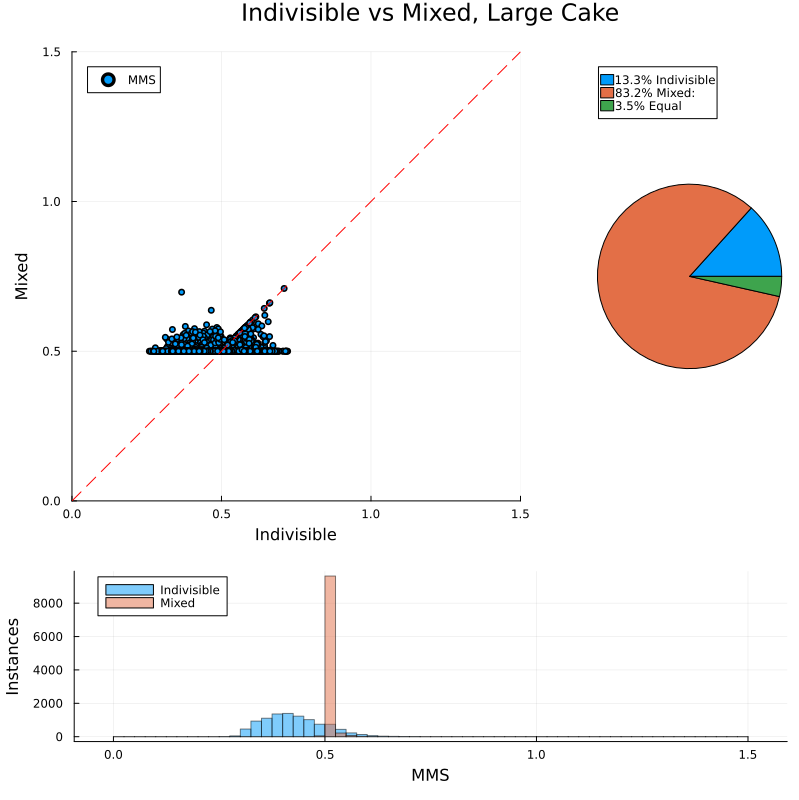
\includegraphics[width=\textwidth]{indivisible_vs_mixed.png}
    \caption{Regular indivisible Algorithm vs Mixed Algorithm.}
    \label{fig:indivisible_vs_mixed}
\end{figure}

\subsection{Cutting the cake}

Now it is time to perform the analysis when cutting the divisible resource into $n$ pieces. We will perform this analysis on all cake variants seperately to more accurately analyze their results.

\begin{figure}
    \centering
    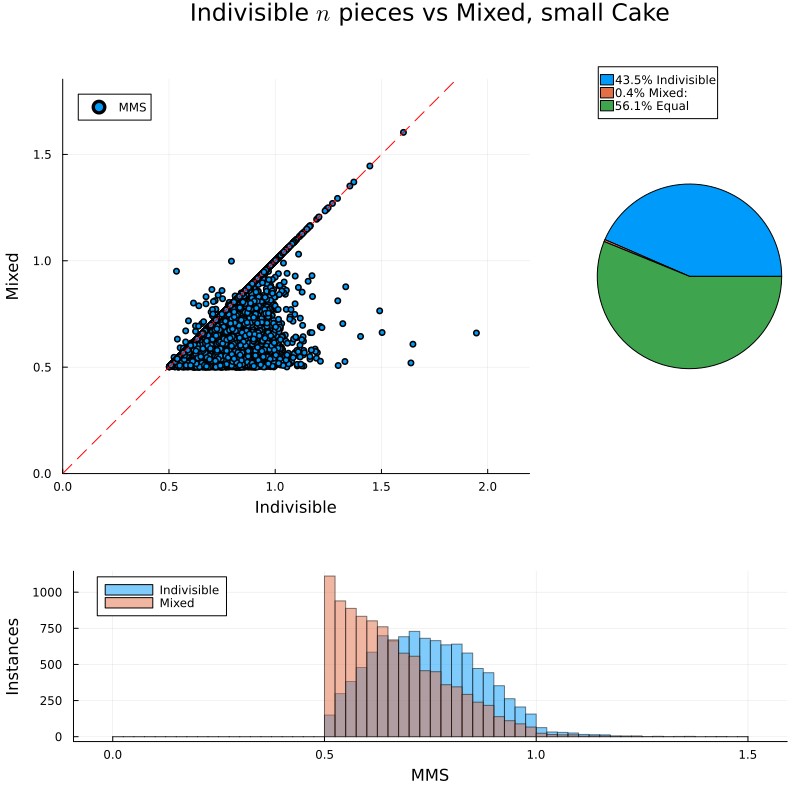
\includegraphics[width=\textwidth]{indivisible_vs_mixed_small.png}
    \caption{Indivisible Algorithm Cutting cake into $n$ pieces vs. Mixed Algorithm for Small Cakes.}
    \label{fig:indivisible_vs_mixed_small}
\end{figure}

We observe in \autoref{fig:indivisible_vs_mixed_small} that as expected, the indivisible algorithm manages to maintain its $\halfMMS$ guarantee as the size of the cake small enough that there really isn't ever any need to cut it anyway. This was shown in a smaller experiment, not included in this report, the the indivisible algorithm managed to maintain its $\halfMMS$ guarantee even without cutting the cake.
\begin{figure}
    \centering
    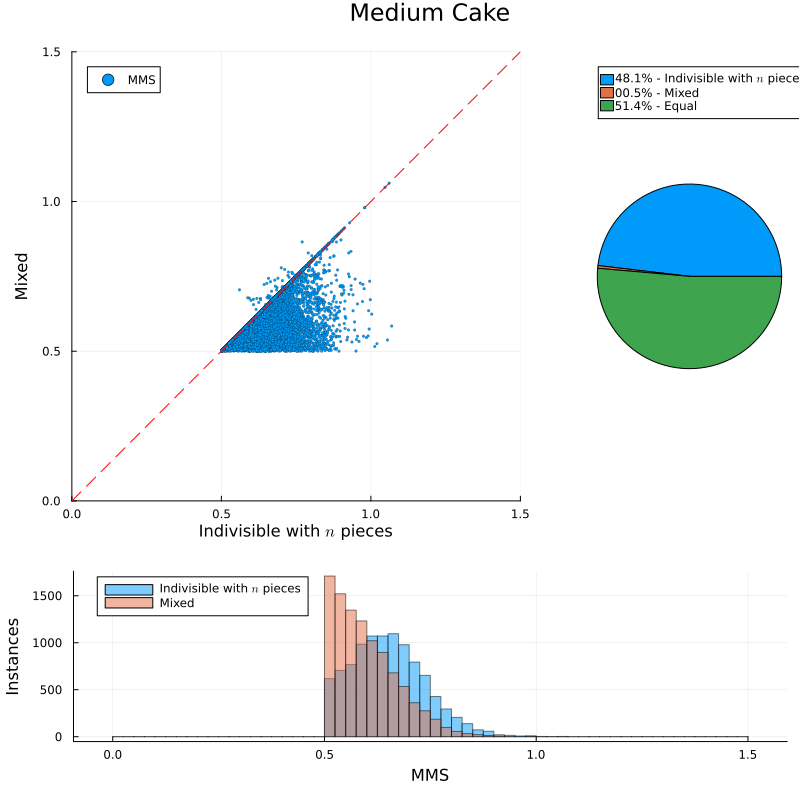
\includegraphics[width=\textwidth]{indivisible_vs_mixed_medium.png}
    \caption{Indivisible Algorithm Cutting cake into $n$ pieces vs. Mixed Algorithm for Medium Cakes.}
    \label{fig:indivisible_vs_mixed_medium}
\end{figure}
In \autoref{fig:indivisible_vs_mixed_medium} not much has changed, but the mixed algorithm has more cake to work with so it is more often able to, and forced to split the cake to achieve $\halfMMS$.
\begin{figure}
    \centering
    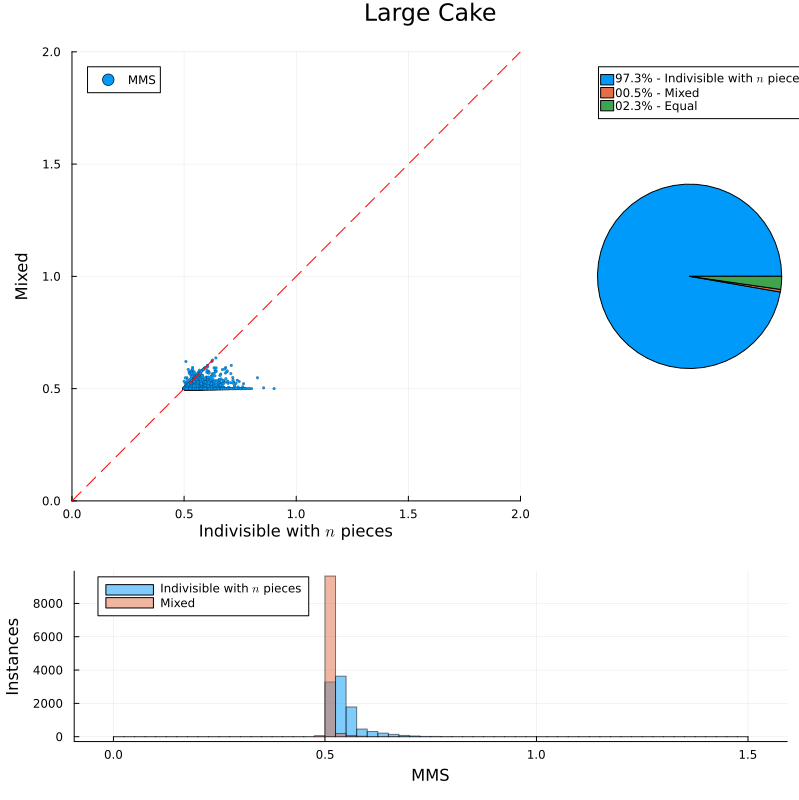
\includegraphics[width=\textwidth]{indivisible_vs_mixed_large.png}
    \caption{Indivisible Algorithm Cutting cake into $n$ pieces vs. Mixed Algorithm for Large Cakes.}
    \label{fig:indivisible_vs_mixed_large}
\end{figure}
AS the cake has grown larger, we see in \autoref{fig:indivisible_vs_mixed_large} that the mixed algorithm is now almost always forced to cut the cake, achieving exactly $\halfMMS$ for the worst bundle.
\begin{figure}
    \centering
    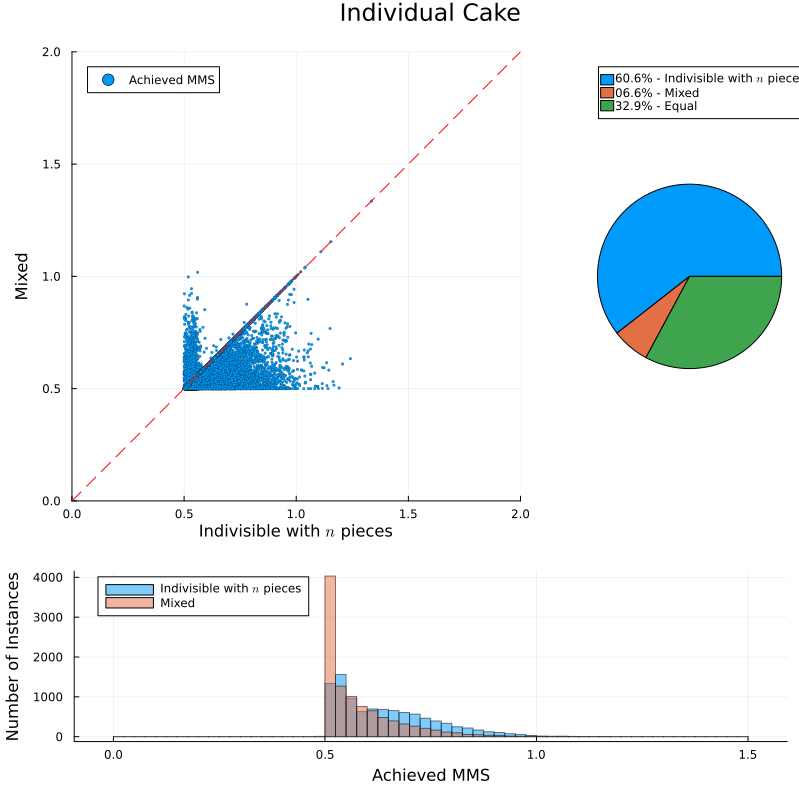
\includegraphics[width=\textwidth]{indivisible_vs_mixed_individual.png}
    \caption{Indivisible Algorithm Cutting cake into $n$ pieces vs. Mixed Algorithm for Individual Cakes.}
    \label{fig:indivisible_vs_mixed_individual}
\end{figure}




\subsubsection{Other Experiments}\label{subsec:other-experiments}
In order to verify that the results of the indivisible algorithm managing to maintain its $\halfMMS$ guarantee aren't exclusive to this exact type of instance, there was also performed a more general analysis on 10 000 instances of varying sizes.

These instances had a random number of agents $n$ where $2\leq\sNumAgents\leq7$, and where the number of goods $\sNumGoods$ were $\sNumAgents\leq\sNumGoods\leq2\sNumAgents$. These limits were set based on the time it takes to allocate these instances for both algorithms. The values were also chosen to ensure these instances cover a more nuanced range of instances, as the main analysis is done on instances were the number of goods could be evenly divided amongst the agents. I limit the instances to have at least $\sNumAgents$ goods, as the indivisible algorithm (without cutting the cake), each agent's MMS allocation would give them an empty bundle as there wouldn't be enough items to go around. This limit could have been removed however when only using the algorithm that cats the cake into $\sNumAgents$ pieces, as this way it would always be at least one slice of cake to each agent.The results of these verifying experiment are shown in \autoref{fig:other_experiments}.

\begin{figure}
    \centering
    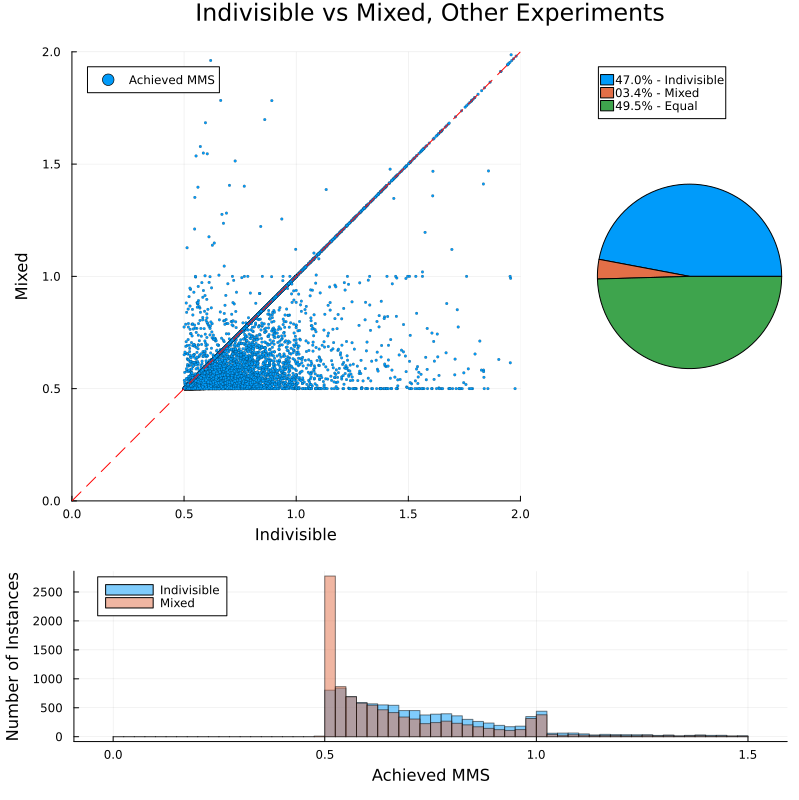
\includegraphics[width=\textwidth]{other_experiments.png}
    \caption{Indivisible Algorithm Cutting cake into $n$ pieces vs. Mixed Algorithm for a wide range of agents and number of goods.}
    \label{fig:other_experiments}
\end{figure}






\subsection{Using Approximated MMS for the Mixed Algorithm}
Next I will perform the same analysis as when comparing the algorithms to compare the results of using a approximated MMS value for the mixed algorithm. The results are shown in \autoref{fig:approximate_vs_exact}.


\begin{figure}
    \centering
    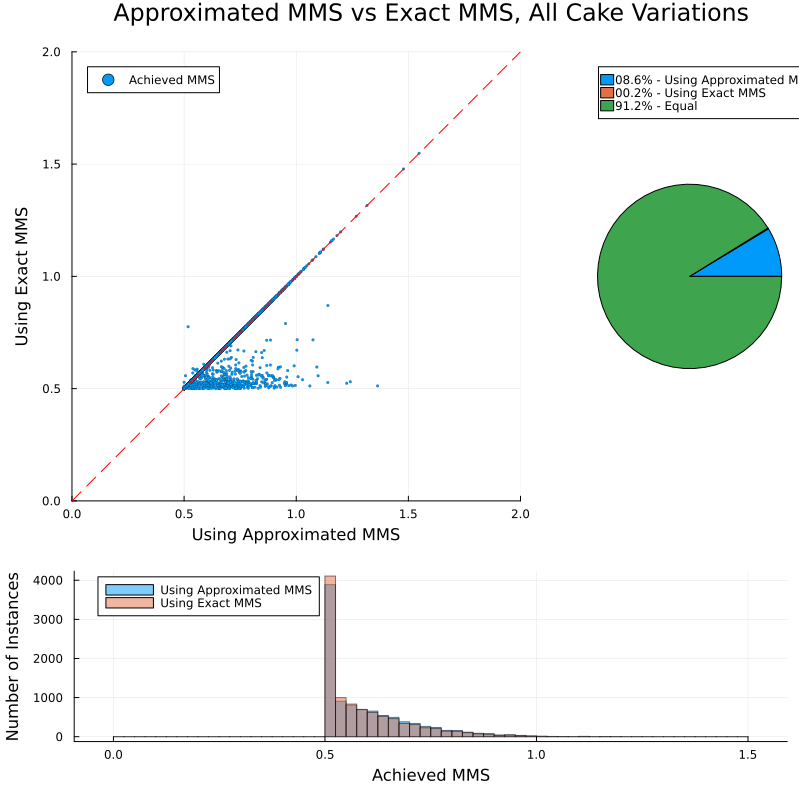
\includegraphics[width=\textwidth]{approximate_vs_exact.png}
    \caption{Approximate vs. Exact MMS calculation for the Mixed Algorithm.}
    \label{fig:approximate_vs_exact}
\end{figure}

Finally a very basic runtime analysis was done for the three variations of algorithms. These results are the average over 10 000 allocations of each type of cake. The results are shown in \autoref{tab:running_time}. Again these experiments are run on instances with $\sNumAgents=4$ and $\sNumGoods=8$. A mor comprehensive analysis should look at how the time is affected by changing the number of agents and goods as well to see how well each algorithm scales along the size of the instance.

% Insert table over running time for the three algorithms
\begin{table}[h]
    \centering
    \caption{Average time each algorithm spent allocating an instance.}
    \label{tab:running_time}
    \begin{tabular}{|l|ccc|}
        \hline
                        & Indivisible $\sNumAgents$ Pieces & Mixed Exact & Mixed Approxmation \\
        \hline
        Small Cake      & 0.138ms                          & 187ms       & 0.00538ms          \\
        Medium Cake     & 0.170ms                          & 129ms       & 0.00215ms          \\
        Large Cake      & 0.148ms                          & 25.0ms      & 0.00589ms          \\
        individual Cake & 0.200ms                          & 121ms       & 0.00252ms          \\
        \hline
    \end{tabular}
\end{table}




\section{Discussion}\label{sec:discussion}


\subsection{Indivisible vs. Mixed Algorithm}
As mentioned in \autoref{chp:introduction}, I initially expected the indivisible algorithm to not be able to maintain its 1/2MMS guarantee, even when cutting the cake into pieces. My expectation was that as the size of the cake pieces get smaller and smaller, the indivisible algorithm will approach the results of the mixed algorithm. My intuition told me that as the number of pieces approached $\infty$, the indivisible algorithm would essentially be turned into an algorithm for divisible goods, albeit an incredibly slow one as a massive instance such as that would require immense computing power and time using the current known algorithms.

The initial results with the purely indivisible cake (\autoref{fig:indivisible_vs_mixed}) seemed to confirm my intuition, in that the algorithm mostly achieves MMS values around 0.4 MMS, and that is with the cake being only the exact sum of the indivisible items, this achieved MMS value would strictly decrease for an instance if the cake would increase in size.

The results from the next experiments were therefore somewhat surprising. Immediately after cutting the cake into $n$ pieces the indivisible algorithm achieves its guarantee, regardless of the size of the cake. We also see as for the small and medium cake both algorithm achieve the exact same $\MMS$ over 50\% of the time which likely mean they find hte exact same allocation. AS the cake gets large though, the indivisible algorithm achieves higher MMS for almost all instances, which is quite surprising as one would expect an indivisible algorithm to perform worse the larger the cake is. The same can be said for the individual cake, where the cake can have any value, which seems to be a good mix of all of the above cases, as it seems it doesn't matter as much if the perceived value of the cake is shared amongst the agents.

Even though these results initially was quite suprising. It is yet to be proven for all instances that an indivisible algorithm will maintain its 1/2MMS guarantee. We can however convince ourselves that they make sense. 

Let us first assume an instance $\sInstance$, has no items, only a cake $\sTheCake$, and the number of agents $\sNumAgents\geq2$, all the agents MMS allocations, and MMS values for $\sInstance$ will simply be their proportional piece of the cake $\sTheCake$, which the indivisible algorithm with $\sNumAgents$ pieces of cake can achieve 1/2MMS easily. Now lets add a single indivisible item $\sItem$ to this instance. If $\sValuation_\sAgent(\sItem)<\sValuation_\sAgent(\sTheCake)/\sNumAgents$ then this good does not affect the MMS value of the agent at all, as this good can simply be given to any other agent. And if $\sValuation_\sAgent(\sItem)\geq\sValuation_\sAgent(\sTheCake)/\sNumAgents$ this will increase the MMS value of the agent, but in return this item is now worth more than a piece of cake and such any agent that receives this item does no longer receive any cake and the MMS value of the agent increases to $\sValuation_\sAgent(\sTheCake)/()\sNumAgents-1)$. This still isn't a problem for the 1/2MMS guarantee though as $\sValuation_\sAgent(\sTheCake)/(\sNumAgents-1)>\frac{1}{2}\sValuation_\sAgent(\sTheCake)/\sNumAgents$ as long as $\sNumAgents>2$. and if the instance only has 2 agents, then the agent that doesn't receive the item can receive more pieces of the cake.

Intuitively it also makes sense as a small and medium cake doesn't necessarily need ot be cut into any pieces as the items will likely be of equal or higher value so the cake doesn't affect the $\MMS$ value much. For large cakes we have the opposite that this means each agents gets at least one piece of the cake, and the remaining items are them split such that the 1/2 MMS is still achieved. A more through theoretical analysis and proof of these theorems are needed, but as the results weren't expected there simply wasn't enough time for such an analysis in this project, but this will be a natural part of future work, in combination with generalizing the conepts for heterogenous cake (and by extenesion multiple cakes).

In order to generalize these findings for heterogenous cake, one could possibly utilize what is  \emph{Weighted Proportional Cake Cutting} as explained in \cite{mms}. This concept generalizes proportionality to the weighted case in cake cutting using a weight profile. This would however require some more pre-processing in order to convert to and from homogenous and heterogenous cakes, which reduces one of the main benefits of simply using a indivisible algorithm directly

Another surpising result is that there seems to be some small subset of variable instances that the mixed algorithm is able to solve better than the indivisible algorithm, despite the indivisible algorithm outperforming for all cake sizes. No further analysis was performer to extract these instances for further analysis as they represented a small percentage of the instances, they are however frequent enough that they should be investigated further. 

In \autoref{fig:other_experiments} we also see how the achieved MMS values for both algorithms has a little spike at $1-MMS$, this is likely due to the randomly created instances creating instances that are easy to give each agent exactly what they expect. This would be instances where all agents have very similar valuations for the items, which is more likely to happen as the number of goods and agents decrease. 



\subsection{Approximation vs Exact}
While the analysis of using $\MMS_\sAgent\approx\PROP_\sAgent$ to approximate the MMS value suffers from some of the same limitations as the indivisible vs mixed analysis. My results indicate, as expected that for most instances this approximation has no real effect on the resulting allocation. This is especially tru for instances with medium, and large cake, as these instances often have such an abundance of cake that it allows each agent to create an MMS allocation where all bundles have the exact same value, which will be equal to $\PROP$, clearly shown in \autoref{fig:allocation_all_mms}.

The use of an exact MMS value is done as per the described algorithm\cite{mms}, with the uncertainty that my implementation may not be the most techincally efficient, the basic runtime analysis show a massive speedup in computation time, with comparable or mostly equal results to using the exact values.


\subsection{Runtime Analysis}
Since the runtime analysis is fairly limited, I would hesitate to draw any major conclusions from their result. However since the mixed algorithm needs hundreds of times longer per instance depending on the instance than the indivisible (while cutting the cake into $n$ pieces), I would argue that the indivisible algorithm outperforms the mixed algorithm in terms of runtime. However when using the approximation of each agents MMS value instead of the exact one, this runtime decreases drastically and is now faster than the indivisible algorithm. This is again not a completely fair comparison as the indivisible algorithm used in this project also handles constraints, while the mixed algorithm does not.
